% Created 2022-04-08 Fri 20:50
% Intended LaTeX compiler: pdflatex
\documentclass[11pt]{article}
\usepackage[utf8]{inputenc}
\usepackage[T1]{fontenc}
\usepackage{graphicx}
\usepackage{longtable}
\usepackage{wrapfig}
\usepackage{rotating}
\usepackage[normalem]{ulem}
\usepackage{amsmath}
\usepackage{amssymb}
\usepackage{capt-of}
\usepackage{hyperref}
\author{Mihir Mahajan}
\date{\today}
\title{Zusammenfassung}
\hypersetup{
 pdfauthor={Mihir Mahajan},
 pdftitle={Zusammenfassung},
 pdfkeywords={},
 pdfsubject={},
 pdfcreator={Emacs 28.1 (Org mode 9.6)}, 
 pdflang={English}}
\begin{document}

\maketitle
\tableofcontents


\section{Statik}
\label{sec:orgb323c77}
\subsection{Grundbegriffe}
\label{sec:org96b79e4}

\subsubsection{Invarianzoperationen Kräftesystem}
\label{sec:org2ca1f1d}
\begin{enumerate}
\item Verschieben einer Kraft in Richtung ihrer Wirkungslinie
\end{enumerate}
(Linienflüchtigkeit von Kräften auf starre Körper)
\begin{enumerate}
\item Zusammenfassen von Kräften mit gemeinsamem Angriffspunkt
\item Zerlegen von Kräften in Komponenten:
\end{enumerate}
\(F_{res} = F_1 + F_2\)
\begin{enumerate}
\item Hinzufügen von Nullkräften:
\end{enumerate}
\(F_1 - F_1 = 0\)
(z.B. zwei entgegengesetzt gerichtete Kräfte mit gleicher Wirkungslinie)

\subsubsection{(Dreh-)Moment}
\label{sec:orgdeec4d9}
\begin{enumerate}
\item Kräftepaar
\label{sec:org1a01c98}
\begin{itemize}
\item Rotation wird als Vektor dargestellt.
\item Richtung über Rechte Hand Regel
\item Länge des Vektors bezeichnet Größe der Rotationswirkung
\item Kann an beliebiger Stelle des Körpers angreifen und ist somit nicht an Wirkungslinie gebunden: \textbf{freier Vektor} (= nicht an Bezugspunkt gebunden)
\item Betrag des Moments M ergbibt sich durch \(M = h*F\), wobei h der senkrechte Abstand der beiden Kräfte ist (F und -F)
\item Greifen mehrere Kräftepaare an so kann man die Momente einfach addieren
\end{itemize}
\item Einzelkraft
\label{sec:org3bcc962}
Eine an einem starren Körper in A angreifende Einzelkraft F vom Betrag F hat die gleiche Wirkung auf den Körper wie die in einen Bezugspunkt B parallel verschobene Kraft und ein Moment \(M_B\) welches den rotationswirksamen Anteil von F bzgl. B angibt.
\begin{itemize}
\item \(\underline{M_B} = r_{BA} \times F \rightarrow |\underline{M_B}| = h*F\)
\end{itemize}
\end{enumerate}
\subsubsection{Gleichgewicht}
\label{sec:orgfc9449c}
Ein Körper ist in der x,y-Ebene im Gleichgewicht wenn die Summe aller Kräfte in jeweils x und y Richtung null sind und die Summe aller Momentvektoren für beliebigen Bezugspunkt 0 ist.

\subsection{Freischneiden}
\label{sec:orgd7ad973}
\subsubsection{Tragwerkskomponente}
\label{sec:org9782ddc}
\begin{itemize}
\item Seil: Bauteil, dessen Querschnittsabmessungen sehr viel kleiner sind als seine
\end{itemize}
Längsabmessung (d << l); nur auf Zug in Richtung seiner Längsachse belastbar
\begin{itemize}
\item Stab: Bauteil, dessen Querschnittsabmessungen sehr viel kleiner sind als seine
\end{itemize}
Längsabmessung (d << l); belastbar auf Zug und Druck, aber nur in Richtung seiner
Längsachse
\begin{itemize}
\item Balken: Bauteil, dessen Querschnittsabmessungen deutlich kleiner sind als seine
\end{itemize}
Längsabmessung (d << l); jedoch in allen Richtungen auf Zug und Druck belastbar
\subsubsection{Lagerräume}
\label{sec:org3195b4f}
\begin{figure}[htbp]
\centering
\includegraphics[width=.9\linewidth]{./img/lagerräume_systeme1.png}
\caption{Lagerräume ebener Systeme}
\end{figure}
\begin{figure}[htbp]
\centering
\includegraphics[width=.9\linewidth]{./img/lagerräume_systeme2.png}
\caption{Lagerräume ebener Systeme}
\end{figure}

\subsubsection{Statische Bestimmtheit}
\label{sec:orge85d95c}
\begin{itemize}
\item Ein n-teiliges mechanisches System heißt statisch bestimmt, wenn alle Lager- und Verbindungsreaktionen eindeutig aus den Gleichgewichtsbedingungen berechenbar sind.
\item Andernfalls heißt es statisch unbestimmt.

\item Die Anzahl möglicher Gleichgewichtsbedingungen ergibt sich als
‘Anzahl der Freiheitsgrade je Teil’ × ‘Anzahl Teile’.
\item Bsp:
\begin{itemize}
\item Im Raum hat jeder Körper 6 Freiheitsgrade (3 × Translation, 3 × Rotation),
\item in der Ebene: 3 Freiheitsgrade (2 × Translation, 1 × Rotation).
\end{itemize}

\item Es muss demnach für ebene n-teilige Systeme gelten:
\textbf{\(r + v = 3n\)}
\end{itemize}

\textbf{In anderen Worten prüfen wie viel wertig jedes Lager ist (r) und wie viele Lager es gibt (v)}

\subsubsection{Haftreibung}
\label{sec:org00a7ce2}
\begin{itemize}
\item \(|F_T| \leq \mu_0 * |F_N|\)
\end{itemize}

\subsection{Schwerpunkt}
\label{sec:org7afca80}
\subsubsection{Schwerpunkt einer Gruppe paralleler Einzelkräfte}
\label{sec:orge6031f1}
Eine Kräftegruppe \(\{F_i\}\) parallel wirkender Einzelkräfte (hier: \(F_i ∥ e_z\)) lässt sich durch eine
resultierende Einzellast R, welche am Schwerpunkt (der Kräftegruppe) \(S = (x_S, y_S)\) angreift
\begin{itemize}
\item \(\underline{R} = \sum_i \underline{F_i}\)
\item \(x_S = \frac{\sum_i x_i F_i}{\sum_i F_i}\)
\item \(y_S = \frac{\sum_i y_i F_i}{\sum_i F_i}\)
\end{itemize}

\subsubsection{Verallgemeinerung auf kontinuierliche Kräfte}
\label{sec:org037f798}
\begin{enumerate}
\item Linienlast
\label{sec:orgc1d21c5}
Sind diese parallelen Kräfte kontinuierlich und nur entlang einer Linie verteilt, so spricht man von einer \textbf{Linienlast} q(x) [N/m].

Diese lässt sich durch eine in \(S_q = {x_S}\) angreifende Einzelkraft \(R_q\) ersetzen, wobei gilt:
\(R_q = \int q(x) dx\), \(x_S = \frac{\int x \ q(x) dx}{R_q}\)
\item Flächenlast
\label{sec:orgb4b406b}
Sind die parallelen Kräfte kontinuierlich über eine Fläche verteilt, so spricht man von einer
Flächenlast \(p(x, y)\) [N/m2] (Druck).
Diese lässt sich durch eine in \(S_P = (x_S, y_S)\) angreifende Einzelkraft P ersetzen, wobei gilt:

\(P = \int p(x,y) dA\), \(x_S = \frac{\int x \ p(x,y) dA}{P}\), \(y_S = \frac{\int y \ p(x,y) dA}{P}\)
\item Volumenkraft
\label{sec:orgc2890c2}
Eine parallel wirkende Volumenkraft f(x, y, z) [N/m3] lässt sich durch eine Einzelkraft F ersetzen, welche in einem Angriffspunkt SF = (xS, yS, zS) angreift, wobei gilt:
\(F = \int f(x,y,z)dV\), \(x_S = \frac{1}{F} \int x \ f(x,y,z)dV\), \(y_S = \frac{1}{F} \int y \ f(x,y,z)dV\), \(z_S = \frac{1}{F} \int z \ f(x,y,z)dV\)

\item Flächenmittelpunkt
\label{sec:orgdbeb15f}

Mittelpunkt bzw geometrischer Schwerpunkt \(S = (x_S, y_S)\) einer ebenen Fläche der Größe A ist definiert durch
\(x_S = \frac{1}{A} \int x dA\)
\(y_S = \frac{1}{A} \int y dA\)

\begin{enumerate}
\item Sonderfälle:
\label{sec:orgbf954a0}
\begin{itemize}
\item Schwerpunkt einer achsensymmetrischen Fläche liegt auf der achse
\item Eine Fläche aus mehreren Teilflächen mit Flächenschwerpunkten \(S_i = (x_i,y_i)\):
\(x_S = \frac{\sum_i x A_i}{\sum_i A_i}\)
\(y_S = \frac{\sum_i y A_i}{\sum_i A_i}\)
\item Löcher zählen als negative Fläche
\end{itemize}

\begin{figure}[htbp]
\centering
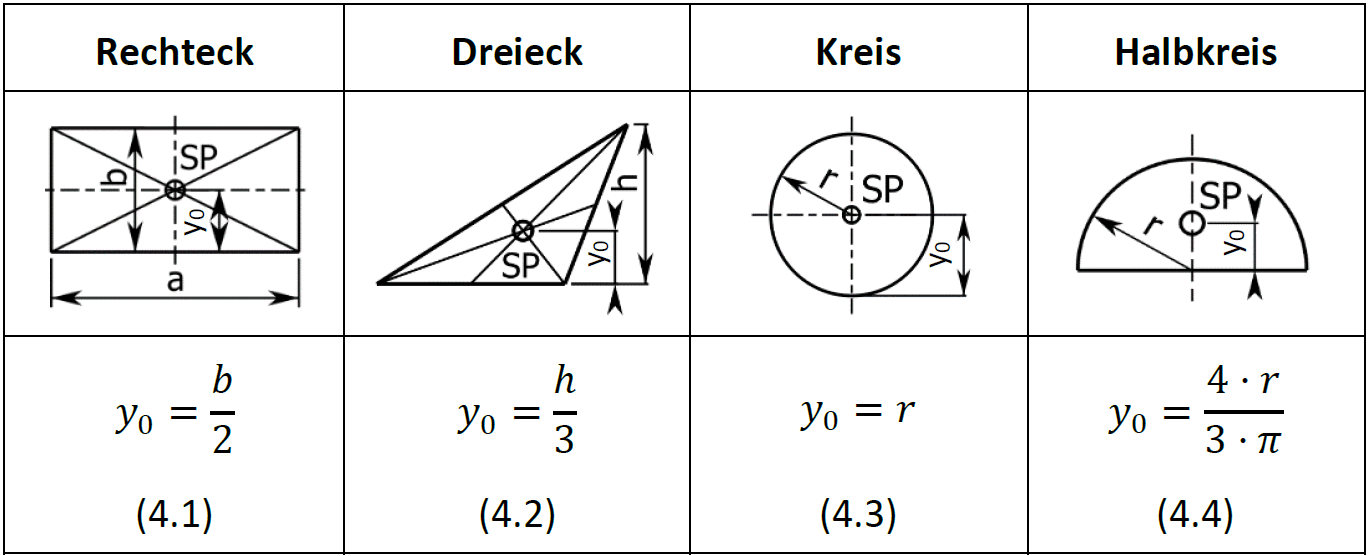
\includegraphics[width=.9\linewidth]{./img/schwerpunkt_tabelle.png}
\caption{Besondere Schwerpunkte}
\end{figure}
\end{enumerate}
\item Volumenmittelpunkt
\label{sec:orgde0908d}
\begin{itemize}
\item \(x_S = \frac{1}{V} \int x dV\)
\item \(y_S = \frac{1}{V} \int y dV\)
\item \(z_S = \frac{1}{V} \int z dV\)
\end{itemize}

Bei homogogener Masseverteilung ist \textbf{Massemittelpunkt = Volumenmittelpunkt}
Sonst Masseverteilungs bzw Dichte verteilung formel

\begin{enumerate}
\item Rotationskörper
\label{sec:orgf6f2659}
\textbf{\(\int z dV = \int_0^z \int_0^{r(z)} \int_0^{2\pi} zr \ d\phi \ dr \ dz\)}
\end{enumerate}
\end{enumerate}
\subsection{Balken}
\label{sec:orgbdcf789}
\subsubsection{Schnittgrößen}
\label{sec:org0574204}
\begin{itemize}
\item Querkraft (senkrecht zur Balkenachse) Q
\item Normalkraft (in Richtung der Balkenachse, normal zur schnittebene) N
\item Biegemoment (y-Komponente des Vektors beschreibt Biegebelastung) M
\end{itemize}
\subsubsection{Einzellasten}
\label{sec:org51b3a3c}
\begin{itemize}
\item Egal WO wir zwischen zwei Einzelkräften schneiden, die Gleichung für das Kräftegleichgewicht bleibt dieselbe, und somit ist die Querkraft zwischen zwei Kraftangriffspunkten \textbf{konstant}.
\item Anders das Moment, welches zwischen den Kraft-Angriffspunkten eine lineare Funktion in x darstellt, und somit dort \textbf{Knicke} aufweist.
\item Am Angriffspunkt einer Einzelkraft F hat also Q(x) einen Sprung (um F), und M(x) einen Knick.
\end{itemize}
\subsubsection{Kontinuierliche Lasten}
\label{sec:org17a14f8}
\begin{itemize}
\item \(\frac{dQ}{dx} = -q(x)\)
\item \(\frac{dN}{dx} = -n(x)\)
\item \(\frac{dM}{dx} = Q(x)\)
\end{itemize}
Integration der differentiellen Zusammenhänge liefert:
\begin{itemize}
\item \(Q(x) = Q(x_0) - \int_{x_0}^{x} q(u) du\)
\item \(M(x) = M(x_0) - \int_{x_0}^{x} Q(u) du\)
\end{itemize}

\subsection{Arbeit, Potential, Stabilität}
\label{sec:orgf3868ea}

\subsubsection{Arbeit}
\label{sec:orgb488236}
Wenn ein Körper mit konstanter Kraft F eine Strecke s verschoben wird so wird Arbeit aufgewand: \(W = F*s\)
Allgemein (also wenn Kraft nicht konstant ist) gilt: \(W = \int_a^b F \ ds\)
Ein Moment, dass einen Körper um einen Winkel \(\phi\) dreht leistet Arbeit: \(W = \int M \ d\phi\)
\subsubsection{Potential}
\label{sec:org917bf01}
Hängt die Arbeit nur von der Lage der Endpunkte der Kraft ab und nicht von der gewählten Bahn so handelt es sich um eine Potentialkraft.
\(\Pi = -W = -\int_a^b F \ ds\)
\begin{enumerate}
\item Beispiele:
\label{sec:orgf220848}
Federpotential: \(\Pi_{Feder} = W_{Feder} = \frac{1}{2} k \Delta x^2\)
Schwerepotential: \(\Pi_{Lage} = W_{Lage} = mgh\)
\end{enumerate}

\subsubsection{Energie}
\label{sec:org6993f5e}
\textbf{Energieerhaltungssatz:}
In einem System ist die Energie am Ende eines Vorgangs gleich groß wie die Energie am Anfang
des Vorgangs, vermehrt um die dem System zugeführte Arbeit und verringert um die vom System
abgeführte Arbeit.
\subsubsection{Stabilität}
\label{sec:org85203cc}
\begin{enumerate}
\item \textbf{stabiles Gleichgewicht:} Bei einer kleinen Störung (Auslenkung) nimmt das Potential des
\end{enumerate}
Systems zu → nach Wegnahme der Störung geht das System in die ursprüngliche Lage
zurück. Kriterium: \(\frac{d^2\Pi}{d^2q} > 0\)
\begin{enumerate}
\item \textbf{indifferentes Gleichgewicht:} Bei einer kleinen Störung verändert sich das Potential des
\end{enumerate}
Systems nicht → nach Wegnahme der Störung bleibt das System in der neuen
Gleichgewichtslage. Kriterium: d2Π/dq2 = d3Π/dq3 = \ldots{} = 0
\begin{enumerate}
\item \textbf{instabiles Gleichgewicht:} Bei einer kleinen Störung nimmt das Potential des Systems ab
\end{enumerate}
→ nach Wegnahme der Störung bewegt sich das System weiter von der alten
Gleichgewichtslage fort. Kriterium: d2Π/dq2 < 0

Ein Zustand / System heißt stabil, wenn sein charakteristisches Verhalten auch bei kleinen
Störungen erhalten bleibt.

\textbf{Systeme mit nur einem Freiheitsgrad q sind somit im Gleichgewicht, wenn gilt: \(\frac{d\Pi}{dq} = 0\)}
\section{Elastostatik}
\label{sec:org08dc46f}
\subsection{Grundbegriffe}
\label{sec:orgc7bf06d}
\subsubsection{Spannung}
\label{sec:orgd6c9f8c}
Normalspannung in einem Körper \(\sigma = \frac{F_N}{A*}\), (negativ: Druckspannung im Körper, positiv: auseinanderziehen im Körper)
Schubspannung in einem Körper \(\tau = \frac{F_T}{A*}\)
\subsubsection{Dehnung}
\label{sec:org9a3b92e}
Dehnung \(\epsilon = \frac{\Delta l}{l_0}\)
\(\epsilon > 0\) Verlängerung, \(\epsilon < 0\) Verkürzung
\begin{enumerate}
\item Ortsabhängige Dehnung
\label{sec:org7e7d736}
Verschiebung u(x)
Differenz von Lage eines materiellen Punktes nach
der Belastung, x + u(x), und ursprünglicher Lage x.
Betrachte differentielles Element der Länge dx an
der Stelle x.

\(\epsilon (x) = \frac{du}{dx}\)
\item Temperatur abhängige Dehnung
\label{sec:orged2af17}
\(\epsilon_T(x) = \alpha * \Delta T(x)\), \(\alpha\) ist Wärmeausdehnungskoeffizient
\end{enumerate}

\subsubsection{Zusammenhang Dehnung und Spannung}
\label{sec:org9d244ef}
Für eindimensionale Probleme (Stäbe) und kleine Dehnungen gilt ein linearer Zusammenhang
zwischen Spannung und elastischem Anteil der Dehnung:
\(\sigma = E * \epsilon_e\) (Hooksches Gesetz)
Analog Feder: \(F = k*\Delta x\)

Unter Wirkung von Spannung + Temperaturänderung
→ Gesamtdehnung = Superposition von spannungsinduzierter und thermischer Dehnung:
    \(\epsilon_{Ges} = \epsilon_e + \epsilon_T = \frac{\sigma}{E} + \alpha \Delta T\)
Für die Verschiebung ergibt sich somit die Differentialgleichung:
\(\frac{du}{dx} = \epsilon_e + \epsilon_T = \frac{N}{EA} + \alpha \Delta T\)
N ist die in Stabrichtung wirkende Kraft (Normalkraft); EA :=Dehnsteifigkeit des Stabs.
\subsubsection{Formänderungsenergie}
\label{sec:org8354170}
\(W = \int dW = \int_0^{\Delta x} F du\)
Bei linear elastischen Stäben gilt: \(F = \frac{EAu}{l} = \sigma * A\)
Also: \(W = \frac{1}{2}Fu\)

\subsection{Spannungszustand}
\label{sec:orgfbbfd1e}
\subsubsection{Spannungstensor}
\label{sec:orga1f1463}
Spannungstensor \(\underline{\underline{\sigma}}(\underline{x}) = \begin{pmatrix}
\sigma_{xx} & \tau_{xy} & \tau{xz}\\
\tau_{yx} & \sigma_{yy} & \tau{yz}\\
\tau_{zx} & \tau{zy} & \sigma_{zz}
\end{pmatrix}\)
Momentengleichgewichte um Achsen durch den Quadermittelpunkt liefern Symmetrie:
\(\tau_{ij} = \tau_{ji} \forall i,j \in \{x,y,z\}\)
Den Spannungsvektor in einer Fläche mit Normale n erhält man damit aus:
\(\underline{t} = \underline{\underline{\sigma^T}} * \underline{n} =  \underline{\underline{\sigma}} * \underline{n}\)
\begin{enumerate}
\item Sonderfall: Ebener Spannungstensor:
\label{sec:orgbc1812b}
\(\underline{\underline{\sigma}} = \begin{pmatrix}
\sigma_{x} & \tau_{xy} \\
\tau_{yx} & \sigma_{y} \\
\end{pmatrix}\)
\end{enumerate}
\subsubsection{{\bfseries\sffamily TODO} Gleichgewichtsbedingungen}
\label{sec:orgc3eec5b}

\subsubsection{Koordinatentransformation}
\label{sec:orgcda05bd}
Gegeben seien zwei Basen eines Vektorraums: \(\{e_x,e_y\}\) und \(\{e_{\xi},e_{\eta}\}\)
Es beschreibe die Matrix \(T = \{a_{ij}\}\) die Darstellung der ξη-Basis als Linearkombination der xy-Basis:
\(\begin{pmatrix} e_{\xi} \\ e_{\eta}\end{pmatrix} = T * \begin{pmatrix} e_{x} \\ e_{y}\end{pmatrix}\)

Transformation eines Ortsvektors: \(P^{xy} \rightarrow P^{\xi \eta}\)

\(P^{\xi \eta} = T *  P^{xy}\)

Sowie für die Transformation von Tensoren, hier am Beispiel des Spannungstensors:

\(\sigma^{\xi \eta} = T * \sigma^{xy} *T^{-1}\)

\begin{enumerate}
\item Spezielle Koordinatentransformation: Ebene Drehung
\label{sec:org3f0725f}

Transformationsmatrix: \(T = \begin{pmatrix}
cos \phi & sin \phi \\
-sin\phi & cos\phi
\end{pmatrix}\)

\(\sigma_\xi = \frac{1}{2}(\sigma_x + \sigma_y) + \frac{1}{2}(\sigma_x - \sigma_y) cos2\phi + \tau_{xy} sin2\phi\)

\(\sigma_\eta = \frac{1}{2}(\sigma_x + \sigma_y) - \frac{1}{2}(\sigma_x - \sigma_y) cos2\phi - \tau_{xy} sin2\phi\)

\(\tau_{\xi \eta} =  - \frac{1}{2}(\sigma_x - \sigma_y) sin2\phi + \tau_{xy} cos2\phi\)
\end{enumerate}
\subsubsection{Hauptspannungen}
\label{sec:orgbb9c8fc}
\begin{enumerate}
\item Hauptrichtung \(\phi^*\)
\label{sec:org3fa23e9}
\(tan2\phi^* = \frac{2\tau_{\xi \eta}}{\sigma_\xi - \sigma_\eta} = \frac{2\tau_{xy}}{\sigma_x - \sigma_y}\)
\item Hauptspannungen
\label{sec:org559cfe0}
Setzt man \(\phi^*\) in die Transformationsgleichungen ein, so ergeben sich die Hauptspannungen \(\sigma_1 > \sigma_2\), die Schubspannungen verschwinden in diesen Richtungen:
\(\sigma_{1,2} = \frac{\sigma_x + \sigma_y}{2} \pm \sqrt{(\frac{\sigma_x - \sigma_y}{2})^2 + \tau_{xy}^2}, \tau_{12} = 0\)
\end{enumerate}
\subsubsection{Mohrscher Spannungskreis}
\label{sec:org12786f6}
Kreisgleichung: \((\sigma - \sigma_M)^2 + \tau^2 = r^2\)
\begin{enumerate}
\item Interpretation
\label{sec:org44d6498}
Normal- und Schubspannungen σ und τ für beliebige Schnitte durch einen Materialpunkt einer
Scheibe liegen in der στ-Ebene auf einem Kreis um σM mit Radius r, dem sogenannten
Mohr’schen Spannungskreis (nach Mohr, 1835-1918).
Der Spannungszustand in einem Punkt einer Scheibe wird also vollständig durch den Mohr’schen
Spannungskreis beschrieben.

\item Konstruktion
\label{sec:org87a3e0f}
\begin{figure}[htbp]
\centering
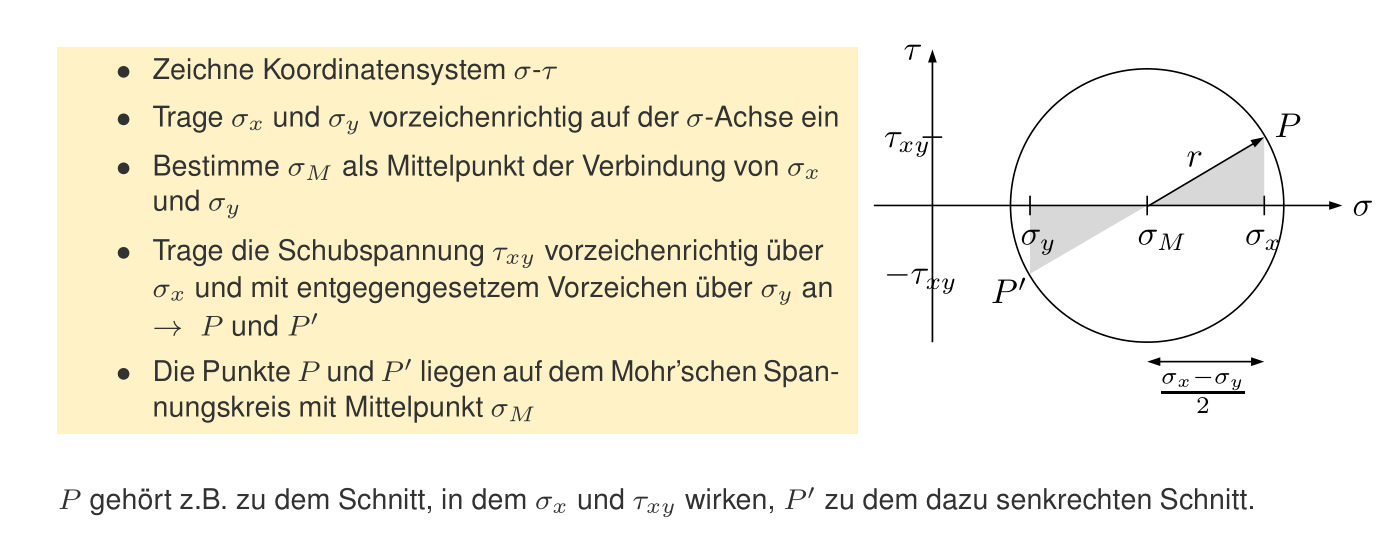
\includegraphics[width=.9\linewidth]{./img/mohrscher_spannungskreis_konstruktion.png}
\caption{Mohrscher Spannungskreis Konstruktion}
\end{figure}
\end{enumerate}

\subsubsection{Verzerrungszustand}
\label{sec:org955296d}
Der Verschiebungsvektor ist der Differenzvektor zwischen der Lage eines Materialelements nach und vor der Verformung:
\(\underline{u}(x,y,z) = \underline{P}´(x,y,z) - \underline{P}(x,y,z)\)

\textbf{Verzerrungstensor}
\(\underline{\underline{\varepsilon}}(x,y,z) = \frac{1}{2}(\Delta \underline{u} + (\Delta \underline{u})^T)\)

\(\varepsilon_{ij} = \frac{1}{2} (\frac{du_i}{d\xi_j} + \frac{du_j}{d\xi_i})\)

\subsubsection{Materialgesetz}
\label{sec:orgf337257}
Zusammenhang zwischen \(\sigma \ und \ \varepsilon\) (Spannungstensor und Verzerrungstensor)

\begin{enumerate}
\item Hooksches Gesetz
\label{sec:org82e699f}
\(\sigma_x = \frac{2G}{1-2\nu}((1-\nu)\epsilon_x + \nu(\epsilon_y+\epsilon_z)), \ \tau_{xy} = 2G\varepsilon_{xy}\)

\(\sigma_y = \frac{2G}{1-2\nu}((1-\nu)\epsilon_y + \nu(\epsilon_x+\epsilon_z)), \ \tau_{yz} = 2G\varepsilon_{yz}\)

\(\sigma_z = \frac{2G}{1-2\nu}((1-\nu)\epsilon_y + \nu(\epsilon_x+\epsilon_y)), \ \tau_{xz} = 2G\varepsilon_{xz}\)

\(E = 2G(1+\nu)\)
\item Berechnung des Spannungszustands
\label{sec:org6d6de63}
\(\sigma_x = \frac{E}{1-v^2}(\varepsilon_x + \nu \varepsilon_y),  \ \tau_{xy} = 2G\varepsilon_{xy}\)

\(\sigma_y = \frac{E}{1-v^2}(\varepsilon_y + \nu \varepsilon_x)\)

\item Berechnung des Verzerrungszustands
\label{sec:orgf5d8712}
\(\varepsilon_x = \frac{1}{E}(\sigma_x - \nu \sigma_y), \ \varepsilon_{xy} = \frac{1}{2G}\tau_{xy}\)

\(\varepsilon_y = \frac{1}{E}(\sigma_y - \nu \sigma_x)\)
\end{enumerate}

\subsubsection{Festigkeitshypothesen}
\label{sec:orga4c961b}
\begin{enumerate}
\item Dimensionskriterien
\label{sec:orgd9023aa}
Vergleichsspannung \(\sigma_V\)

\(\sigma_V \leq \sigma_{zul} = \frac{\sigma_{Grenz}}{S}\)
\item maximale Normalspannung (Rankine)
\label{sec:org2851df0}
\(\sigma_V = \sigma_{max} =\) betragsmäßig maximale Hauptnormalspannung

Eignung: gut für spröden Bruch senkrecht zu \(\sigma_{max}\), nicht geeignet für Plastifizierung

\item maximale Schubspannung (Tresca)
\label{sec:org4233343}
\(\sigma_V = 2\tau_{max} =\) 2 * maximale Schubspannung
Eignung: gut für Plastifizierung (unter BEerücksichtigung der Lage von \(\sigma_M\), sh. Mohr’scher Kreis)

\item maximale Gestaltänderungsenergie (Mises)
\label{sec:orgff0501e}
Liefert schließlich basierend auf den Hauptspannungen \(\sigma_1 \geq \sigma_2 \geq \sigma_3\)
\(\sigma_V = \sqrt{\frac{1}{2} [(\sigma_1 - \sigma_2)^2 + (\sigma_1 - \sigma_3)^2 + (\sigma_2 - \sigma_3)^2]}\)
Eignung: bis heute die (insbesondere für Plastifizierung) am besten funktionierende Hypothese
\end{enumerate}

\subsection{Biegebalken}
\label{sec:org69e97da}
\subsubsection{Verzerrung und Materialgesetz}
\label{sec:org7b47fe3}
\begin{itemize}
\item geometrische Beziehung: \(u(x,z) = \psi (x) * z\)
\item \(\sigma = \sigma_x = E \varepsilon_x = E\psi'z = \frac{M}{I}z\)
\item \(\tau = \tau_{xz} = 2G\varepsilon_{xz} = G(\omega'+\psi)\) (\(\omega\) ist Neigung der verformten Balkenachse (lokal))
\end{itemize}
\subsubsection{Schnittgrößen und Spannungsgrößen}
\label{sec:orgd30fd69}
\begin{itemize}
\item \(Q = \int \tau dA = \int G(\omega' + \psi) dy dz = GA_s (\omega' + \psi)\) (A:= Schubfläche, AG:=Schubsteifigkeit)
\item \(N = \int \sigma dA = E\psi' \int z^2 dA = EI\psi'\) mit \(I = I_y = \int z^2 dA\) (I:= Flächenträgheitsmoment bzgl der y-Achse, EI:=Biegesteifigkeit)
\item \(M = M_y = \int z\sigma \ dA\)
\end{itemize}

\subsubsection{Flächenträgheitsmoment}
\label{sec:org956b63d}
\(I_y = \int z^2 dA\) (axiales FTM bzgl y-Achse)

\(I_z = \int y^2 dA\) (axiales FTM bzgl z-Achse)

\(I_{yz} = I{zy} = -\int yz dA\) (Deviationsmoment)

Die Größe der Flächenträgheitsmomente ist von der Lage des Ursprungs und von der Richtung der Achsen abhängig.
Das Deviationsmoment verschwindet, Iyz = 0, falls y oder z Symmetrieachse ist.

\begin{enumerate}
\item Zusammengesetzte Flächen
\label{sec:org5de7370}
\(A = \sum_i A_i\), \(I_* = \sum_i I_*^{(i)}\)
\item Parallele Koordinatensysteme (Satz von Steiner)
\label{sec:org8f85d18}
Bei parallelen KoSys gilt: \(\bar{y} = y + \bar{y}_S , \bar{z} = z + \bar{z}_S\)
\begin{itemize}
\item \(I_\bar{y} = I_y +\bar{z}_S^2 A\)
\item \(I_\bar{z} = I_z +\bar{y}_S^2 A\)
\item \(I_\bar{yz} = I_{yz} +\bar{y}_S^2  \bar{z}_S^2A\)
\end{itemize}

\item Flächenträgheitsmomente einiger Geometrien:
\label{sec:org3f22e77}
\begin{figure}[htbp]
\centering
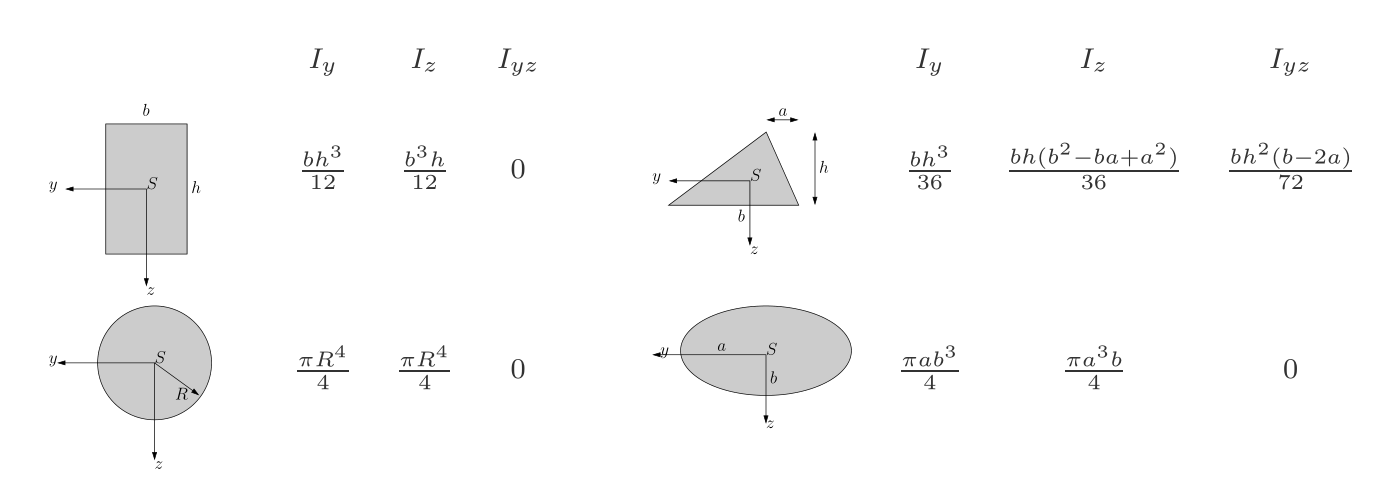
\includegraphics[width=.9\linewidth]{./img/ftm.png}
\caption{Flächenträgheitsmomente einiger Geometrien}
\end{figure}

\item Rotierte KoSy Flächenträgheitstensor
\label{sec:org52c6021}
\(\underline{\underline{I}} = \begin{pmatrix}
I_y & I_{yz} \\
I_{zy} & I_z
\end{pmatrix}\)


\(\underline{\underline{I}}^{\eta \zeta} = \underline{T} * \underline{I}^{yz} * \underline{T}^-1}\)

\begin{itemize}
\item \(I_\eta = \frac{1}{2}(I_y + I_z) + \frac{1}{2}(I_y-I_z) cos(2\varphi) + I_{yz} sin(2\varphi)\)
\item \(I_\zeta = \frac{1}{2}(I_y + I_z) - \frac{1}{2}(I_y-I_z) cos(2\varphi) - I_{yz} sin(2\varphi)\)
\item \(I_\zeta = - \frac{1}{2}(I_y-I_z) sin(2\varphi) - I_{yz} cos(2\varphi)\)
\end{itemize}

\item Hauptträgheitsmomente
\label{sec:org384f1b8}
\(tan2\varphi^* = \frac{2I_{yz}}{I_y - I_z}\)


\(I_{1,2} = \frac{I_y + I_z}{2} \pm \sqrt{(\frac{I_y - I_z}{2})^2 + I_{yz}^2}\), \(I_{12} = 0\)
\end{enumerate}

\subsection{Bernoullibalken}
\label{sec:orgfd38d5c}
\subsubsection{Hypothesen}
\label{sec:org65fcbb3}
\begin{enumerate}
\item Bernoullihypothese:
Die Balkenquerschnitte bleiben unter der Deformation eben, und Ihre Form bleibt erhalten (w unabhängig von z, s.u.) → N = 0
\item Bernoullihypothese:
Querschnitte, die vor der Deformation senkrecht auf der Balkenachse standen, stehen auch nach der Belastung noch senkrecht auf der deformierten Balkenachse (schubstarrer Balken) → \(\frac{dw}{dx} = \omega' \sim -\psi(x)\)
\end{enumerate}
\subsubsection{Biegelinie \(\omega(x)\)}
\label{sec:orgc9c2629}
\(\omega''(x) = -\frac{M(x)}{EI} \sim \kappa\)
, mit \(\kappa\) ist die \textbf{Krümmung} der Biegelinie welche für kleine Durchbiegungen ca. \(\omega''(x)\) ist
\begin{itemize}
\item \(EI\omega''(x) = -M(x)\)
\item \(EI\omega'''(x) = -Q(x)\)
\item \(EI\omega^{(4)} = q(x)\)
\end{itemize}
\subsubsection{Randbedingungen}
\label{sec:orge7f3a63}
\#+CAPTION Einige Randbedingungen
\begin{center}
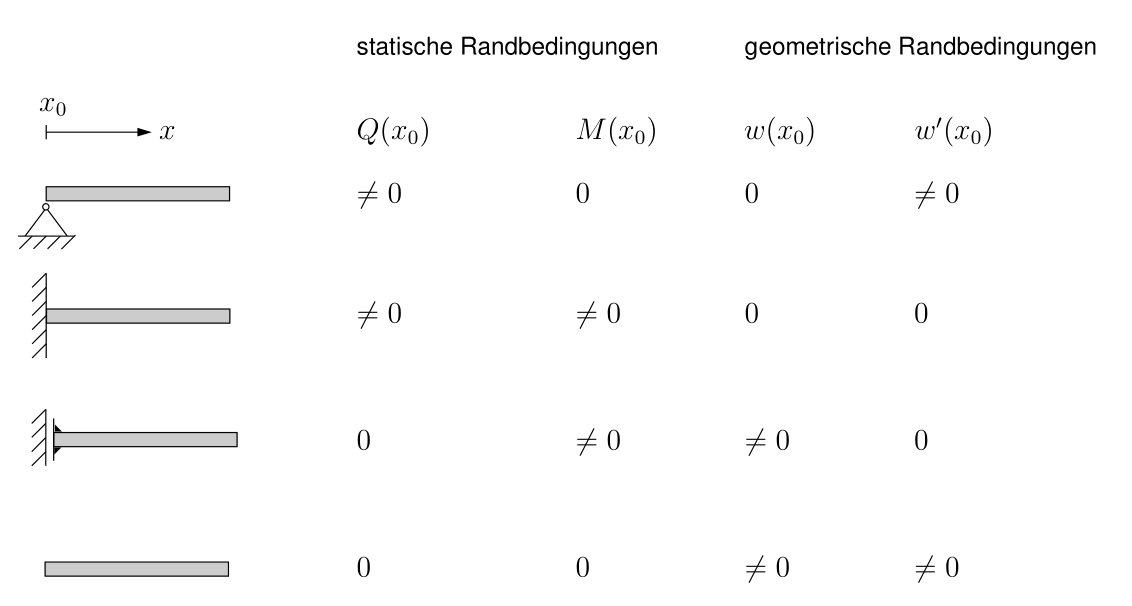
\includegraphics[width=.9\linewidth]{./img/randbedingungen.png}
\end{center}

\section{Kinetik}
\label{sec:org6036426}
\subsection{Kinematik eines Massepunktes}
\label{sec:org21a2187}
\subsubsection{Grundbegriffe}
\label{sec:org865d58b}
\begin{itemize}
\item Ortsvektor \(r(t) = \begin{pmatrix}x(t)\\ y(t)\\ z(t)\end{pmatrix}\)
\item Geschwindigkeit \(v(t) = \begin{pmatrix}x'(t)\\ y'(t)\\ z'(t)\end{pmatrix}\)
\item Beschleunigung \(a(t) = \begin{pmatrix}x''(t)\\ y''(t)\\ z''(t)\end{pmatrix}\)

\item Betrag eines Vektors: \(|\begin{pmatrix}x \\ y \\ z \end{pmatrix}| = \sqrt{x^2+y^2+z^2}\)
\end{itemize}

\subsubsection{geradlinige Bewegung}
\label{sec:org890ae88}
\begin{itemize}
\item gleichförmige Bewegung (konstante Geschwindigkeit): \(x(t) = x_0 + v_0(t-t_0)\), (Liniear)
\item gleichmäßig beschleuningte Bewegung (konstante Beschleunigung): \(x(t) = x_0 + v_0(t-t_0) + \frac{1}{2} a_0 (t-t_0)^2\) (Parabel förmig)
\item zeitabhängig beschleunigte Bewegung: \(v(t) = v(t_0) + \int_{t_0}^t a(\tilde{t}) d \tilde{t}\),  \(x(t) = x(t_0) + \int_{t_0}^t v(\tilde{t}) d \tilde{t}\)
\end{itemize}

\subsubsection{Polarkoordinaten}
\label{sec:org3dc2ab3}
\(\underline{e'_r} = \varphi' \underline{e_{\varphi}}\), \(\underline{e'_\varphi} = -\varphi' \underline{e}_r\)
\begin{itemize}
\item Ortsvektor: \(\underline{r(t)} = r(t) * \underline{e_r}\)
\item Geschwindigkeit: \(\underline{v(t)} = r' * \underline{e_r} + r\varphi' \underline{e_\varphi}\)
\item Beschleunigung: \(\underline{a(t)} = (r''-r\varphi'^2) * \underline{e_r} + (r\varphi'' + 2r'\varphi') \underline{e_\varphi}\)
\item \(\omega = \varphi'\)
\end{itemize}

\subsubsection{Kreisbewegung}
\label{sec:org95b5a48}
\begin{itemize}
\item \(v_\varphi = \bar{r}\omega\)
\item \(a_\varphi = r\omega'\)
\item \(a_r = - r\omega^2\)
\end{itemize}

\subsubsection{Newtonsche Gesetze}
\label{sec:orge8b12c8}
Impuls: \(\underline{p} = m\underline{v}\)

\begin{enumerate}
\item Wenn auf einen Massenpunkt keine Kraft wirkt, so ist der Impuls konstant.
\item Die zeitliche Änderung des Impulses ist gleich der auf den Massenpunkt wirkenden Kraft. \(F = ma = \frac{dp}{dt}\)
\item actio = reactio
\end{enumerate}

\subsubsection{Freie Bewegung}
\label{sec:orge9a96e0}
Einfach intuitiv F=ma drauf klatschen

\subsubsection{Trockene Reibung}
\label{sec:org1f9ad0c}
\(R = N\mu\)
\subsubsection{Widerstand im Fluid bei kleinen Geschwindigkeiten}
\label{sec:org15f7448}
\begin{itemize}
\item \(F_W = kv\)
\item \(F_W^{Strokes} = 6\pi\nu rv\)
\end{itemize}

\subsection{Stoßprozesse}
\label{sec:orgf57e776}
\subsubsection{zeitlicher Ablauf}
\label{sec:orgb6ed109}
\begin{itemize}
\item Kompressionsperiode: \(\hat{F_K} = \int_{t_0}^{t_M} F(t)dt\)
\item Restitutionsperiode: \(\hat{F_R} = \int_{t_;}^{t_{end}} F(t)dt\)
\end{itemize}

\subsubsection{Stoßvorgänge}
\label{sec:org8b96a52}
\begin{itemize}
\item elastischer Stoß (Billiard) \(\hat{F}_K = \hat{F}_R\)
\item teilelastischer Stoß: Teil der kintischen Energie wird in Schwingung oder bleibende Verformung umgewandelt
\item ideal plastischer Stoß: Nur verformung
\end{itemize}

\#+CAPTION zentraler Stoß mit glatten Wand
\begin{center}
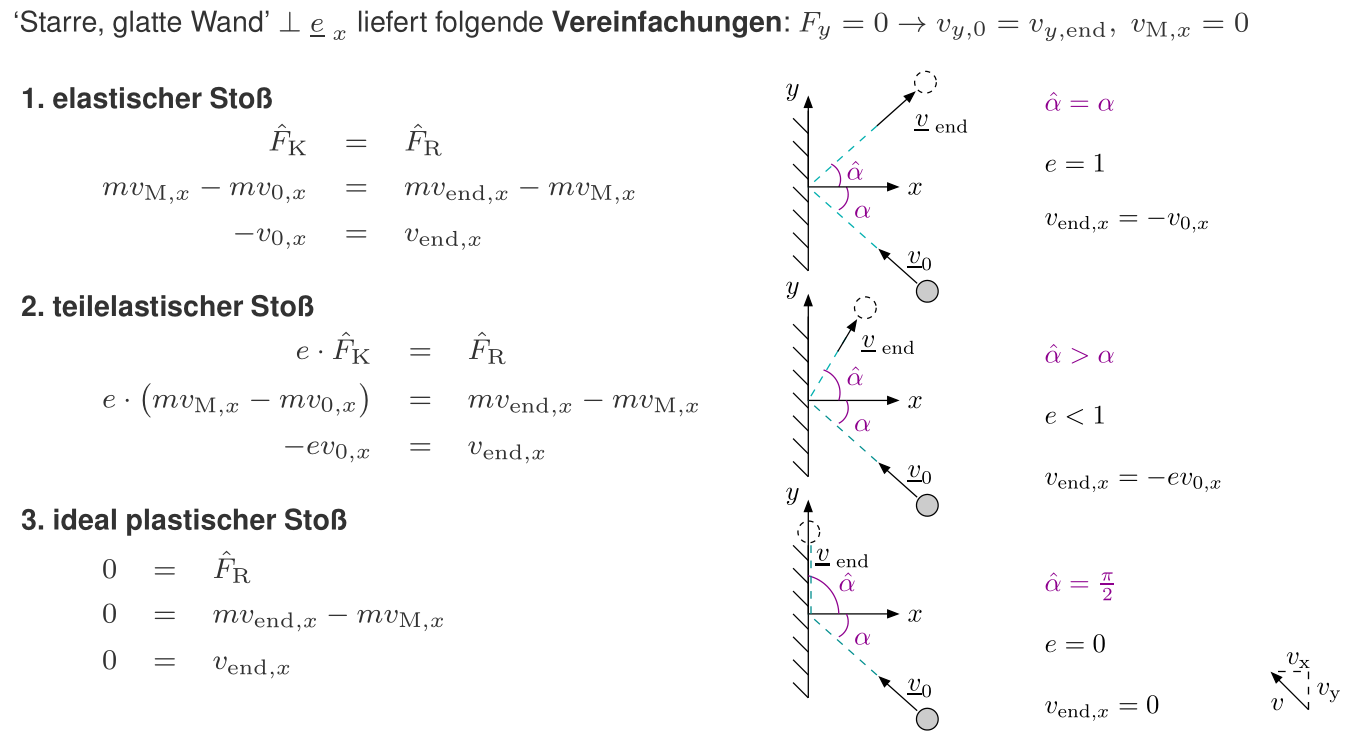
\includegraphics[width=.9\linewidth]{./img/stoßvorgänge.png}
\end{center}
\subsubsection{Impulssatz}
\label{sec:org2a32d87}
\begin{itemize}
\item Kraftstoß: \(\hat{F} = \int_{t_0}^{t_{end}} Fdt\)
\item Impulssatz: \(\hat{F} = mv(t_{end}) - mv(t_0)\)
\end{itemize}

\subsubsection{Systeme von Massepunkten}
\label{sec:org3e3cb84}
\begin{itemize}
\item Schwerpunktsatz: \(m_{ges}\underline{a}_S = \underline{F}_{ext} = \sum_{i=1}^N F_i\)
\item Impulssatz: \(\hat{\underline{F}}_{ext} = m_{ges} \underline{v}_S(t_{end}) - m_{ges} \underline{v}_S(t_0)\), mit \(v_S = \frac{\sum_i(m_i v_i)}{\sum_i m_i}\)
\end{itemize}

\subsubsection{Drallsatz}
\label{sec:org4a3e141}
Drehimpuls \(\underline{L} = \underline{r} \times \underline{p}\)

Aus dem 2ten Newtonschen gesetz:
\(\underline{r} \times \underline{p}' = \underline{r} \times \underline{F} \rightarrow \underline{L}' = \underline{M}\)

\subsubsection{Körper mit veränderlicher Masse}
\label{sec:orgfa931ff}
\(F = ma + m'a\)
\end{document}
